\documentclass[lang=cn,newtx,10pt,scheme=chinese]{elegantbook}

\title{Private Set Intersection}
\subtitle{安全多方计算应用}

\author{牛午甲 \& 潘云石 \& 石磊鑫 \& 孙霄鹍 \& 陈昊}
\institute{USTC}
\date{\today}
\version{0.1}
\bioinfo{}{}

\extrainfo{注意:本模板自 2023 年 1 月 1 日开始,不再更新和维护!}

\setcounter{tocdepth}{3}

\logo{logo-blue.png}
\cover{cover.jpg}

% 本文档命令
\usepackage{array}
\newcommand{\ccr}[1]{\makecell{{\color{#1}\rule{1cm}{1cm}}}}

% 修改标题页的橙色带
\definecolor{customcolor}{RGB}{32,178,170}
\colorlet{coverlinecolor}{customcolor}
\usepackage{cprotect}

\addbibresource[location=local]{reference.bib} % 参考文献,不要删除

\begin{document}
	
\maketitle
\frontmatter

\tableofcontents

\mainmatter
\setcounter{chapter}{-1}
\chapter{数学基础}
\section{数论基础}
\begin{introduction}
	\item 中国剩余定理~\ref{thm:CRT}
	\item Fubini 定理~\ref{thm:fubi}
	\item 最优性原理~\ref{pro:max}
	\item 柯西列性质~\ref{property:cauchy}
	\item 韦达定理
\end{introduction}
\subsection{中国剩余定理}
\begin{theorem}[中国剩余定理, Chinese Remainder Theorem, CRT]\label{thm:CRT}
	设$m_1, m_2,...,m_k$是$k$个两两互素的正整数,$m=m_1m_2\cdots m_k$,记$m=m_iM_i(i=1,2,...,k)$,则同余式组$$x\equiv b_1(mod\ m_1),x\equiv b_2(mod\ m_2),...,x\equiv b_k(mod\ m_k)$$
	有唯一解$$x\equiv M_1'M_1b_1+M_2'M_2b_2+\cdots+M_k'M_kb_k(mod\ m)$$
	其中 $M_i'M_i\equiv 1(mod\ m_i)(i=1,2,...,k)$.
\end{theorem}
\begin{proof}
	证明:
\end{proof}

\begin{corollary}\label{thm:EX_CRT}
	设$m_1, m_2,...,m_k$是$k$个两两互素的正整数,$m=m_1m_2\cdots m_k$,则同余式$f(x)\equiv 0(mod\ m)$有解的充分必要条件是同余式$f(x)\equiv 0(mod\ m_i)(i=1,2,...,k)$每一个都有解,并且若用$T_i$表示$f(x)\equiv 0(mod\ m_i)$的解数,$T$表示$f(x)\equiv 0(mod\ m)$的解数,则$T=T_1T_2\cdots T_k$.
\end{corollary}
\begin{proof}
	证明
\end{proof}

\section{抽象代数基础}

\chapter{基础知识介绍}

\begin{introduction}
	\item Rabin不经意传输协议~\ref{def:Rabin}
	\item Fubini 定理~\ref{thm:fubi}
	\item 最优性原理~\ref{pro:max}
	\item 柯西列性质~\ref{property:cauchy}
	\item 韦达定理
\end{introduction}

\section{不经意传输(Oblivious transfer,OT)}
\textbf{不经意传输(Oblivious transfer,OT)}是密码学中的一类协议,实现了发送方将潜在的许多信息中的一个传递给接收方,但但事后对发送了哪一条消息给接收方保持未知状态。

\subsection{Rabin不经意传输协议}
不经意传输最早由Michael O. Rabin在1981年提出。在这种形式下,发送方以$\frac{1}{2}$的概率向接收方发送一个信息,而发送方不知道接收方是否收到该信息,只有接收方能确信地知道自己是否收到了消息。Rabin的方案是基于RSA的。
在介绍Rabin的方案之前,需要介绍几个模平方根相关的引理。
\begin{lemma}
	若$m_1,m_2,...,m_k$是$k$个
\end{lemma}
\begin{definition}[Rabin's oblivious transfer protocol] \label{def:Rabin} 
	准备工作:Alice 按照RSA算法生成模数$N=pq$(这里$p,q$是大素数)、指数$e$(要保证$e$和$r=(p-1)(q-1)$互素)。
\begin{enumerate}
	\item Alice 发送$N,e,m^e\ mod\ N$给 Bob;
	\item\label{two} Bob 选择随机数$x$,将$x^2\ mod\ N$发给 Alice;
	\item Alice 求解$x^2\ mod\ N$的四个平方根,选择其中一个(记作$y$)发给 Bob;
\end{enumerate}
	如果 Bob 发现 $y\ mod\ N$ 既不等于 $x\ mod\ N$ 也不等于 $-x\ mod\ N$,那么Bob就可以对 $N$ 进行素因子分解得到 $p,q$ ,从而求得$r$。然后 Bob 求解$ed\equiv 1\ mod\ r$ 得到$d$,再解密$m^{ed}\ mod\ N$获得$m$的明文。然而,如果$y\ mod\ N$ 是 $x\ mod\ N$ 和 $-x\ mod\ N$中的一个,那么Bob就无法分解$N$,从而不能解密得到明文。
\end{definition}
\begin{remark}
	对上述协议需要做几点说明:
\begin{enumerate}
	\item 在协议第~\ref{two}步中,由于 $N$ 的素因子只有 $p,q$,并且 $N$ 非常大,因此认为 $x$ 和 $N$ 互素,从而$x^2\ mod\ N$有四个平方根。
	\item 
\end{enumerate}
\end{remark}

\begin{corollary}[推论名称] \label{thm:Rabin} 
	推论内容
\end{corollary}


\subsection{1-2不经意传输}


\begin{definition}[定义名称] \label{def:int} 
	定义内容
	\begin{equation}
		换行公式
	\end{equation}
\end{definition}

\begin{exercise}\label{exer:43}
	练习
\end{exercise}

\begin{solution}
	解
\end{solution}

\begin{remark}
	注
\end{remark}

\begin{proof}
	证明
\end{proof}

\begin{theorem}[定理名称] \label{thm:fubi} 
	定理内容
\end{theorem}

\begin{note}
	笔记
\end{note}

\begin{proposition}[命题名称] \label{pro:max}
	命题内容
\end{proposition}

图片
\begin{figure}[htbp]
	\centering
	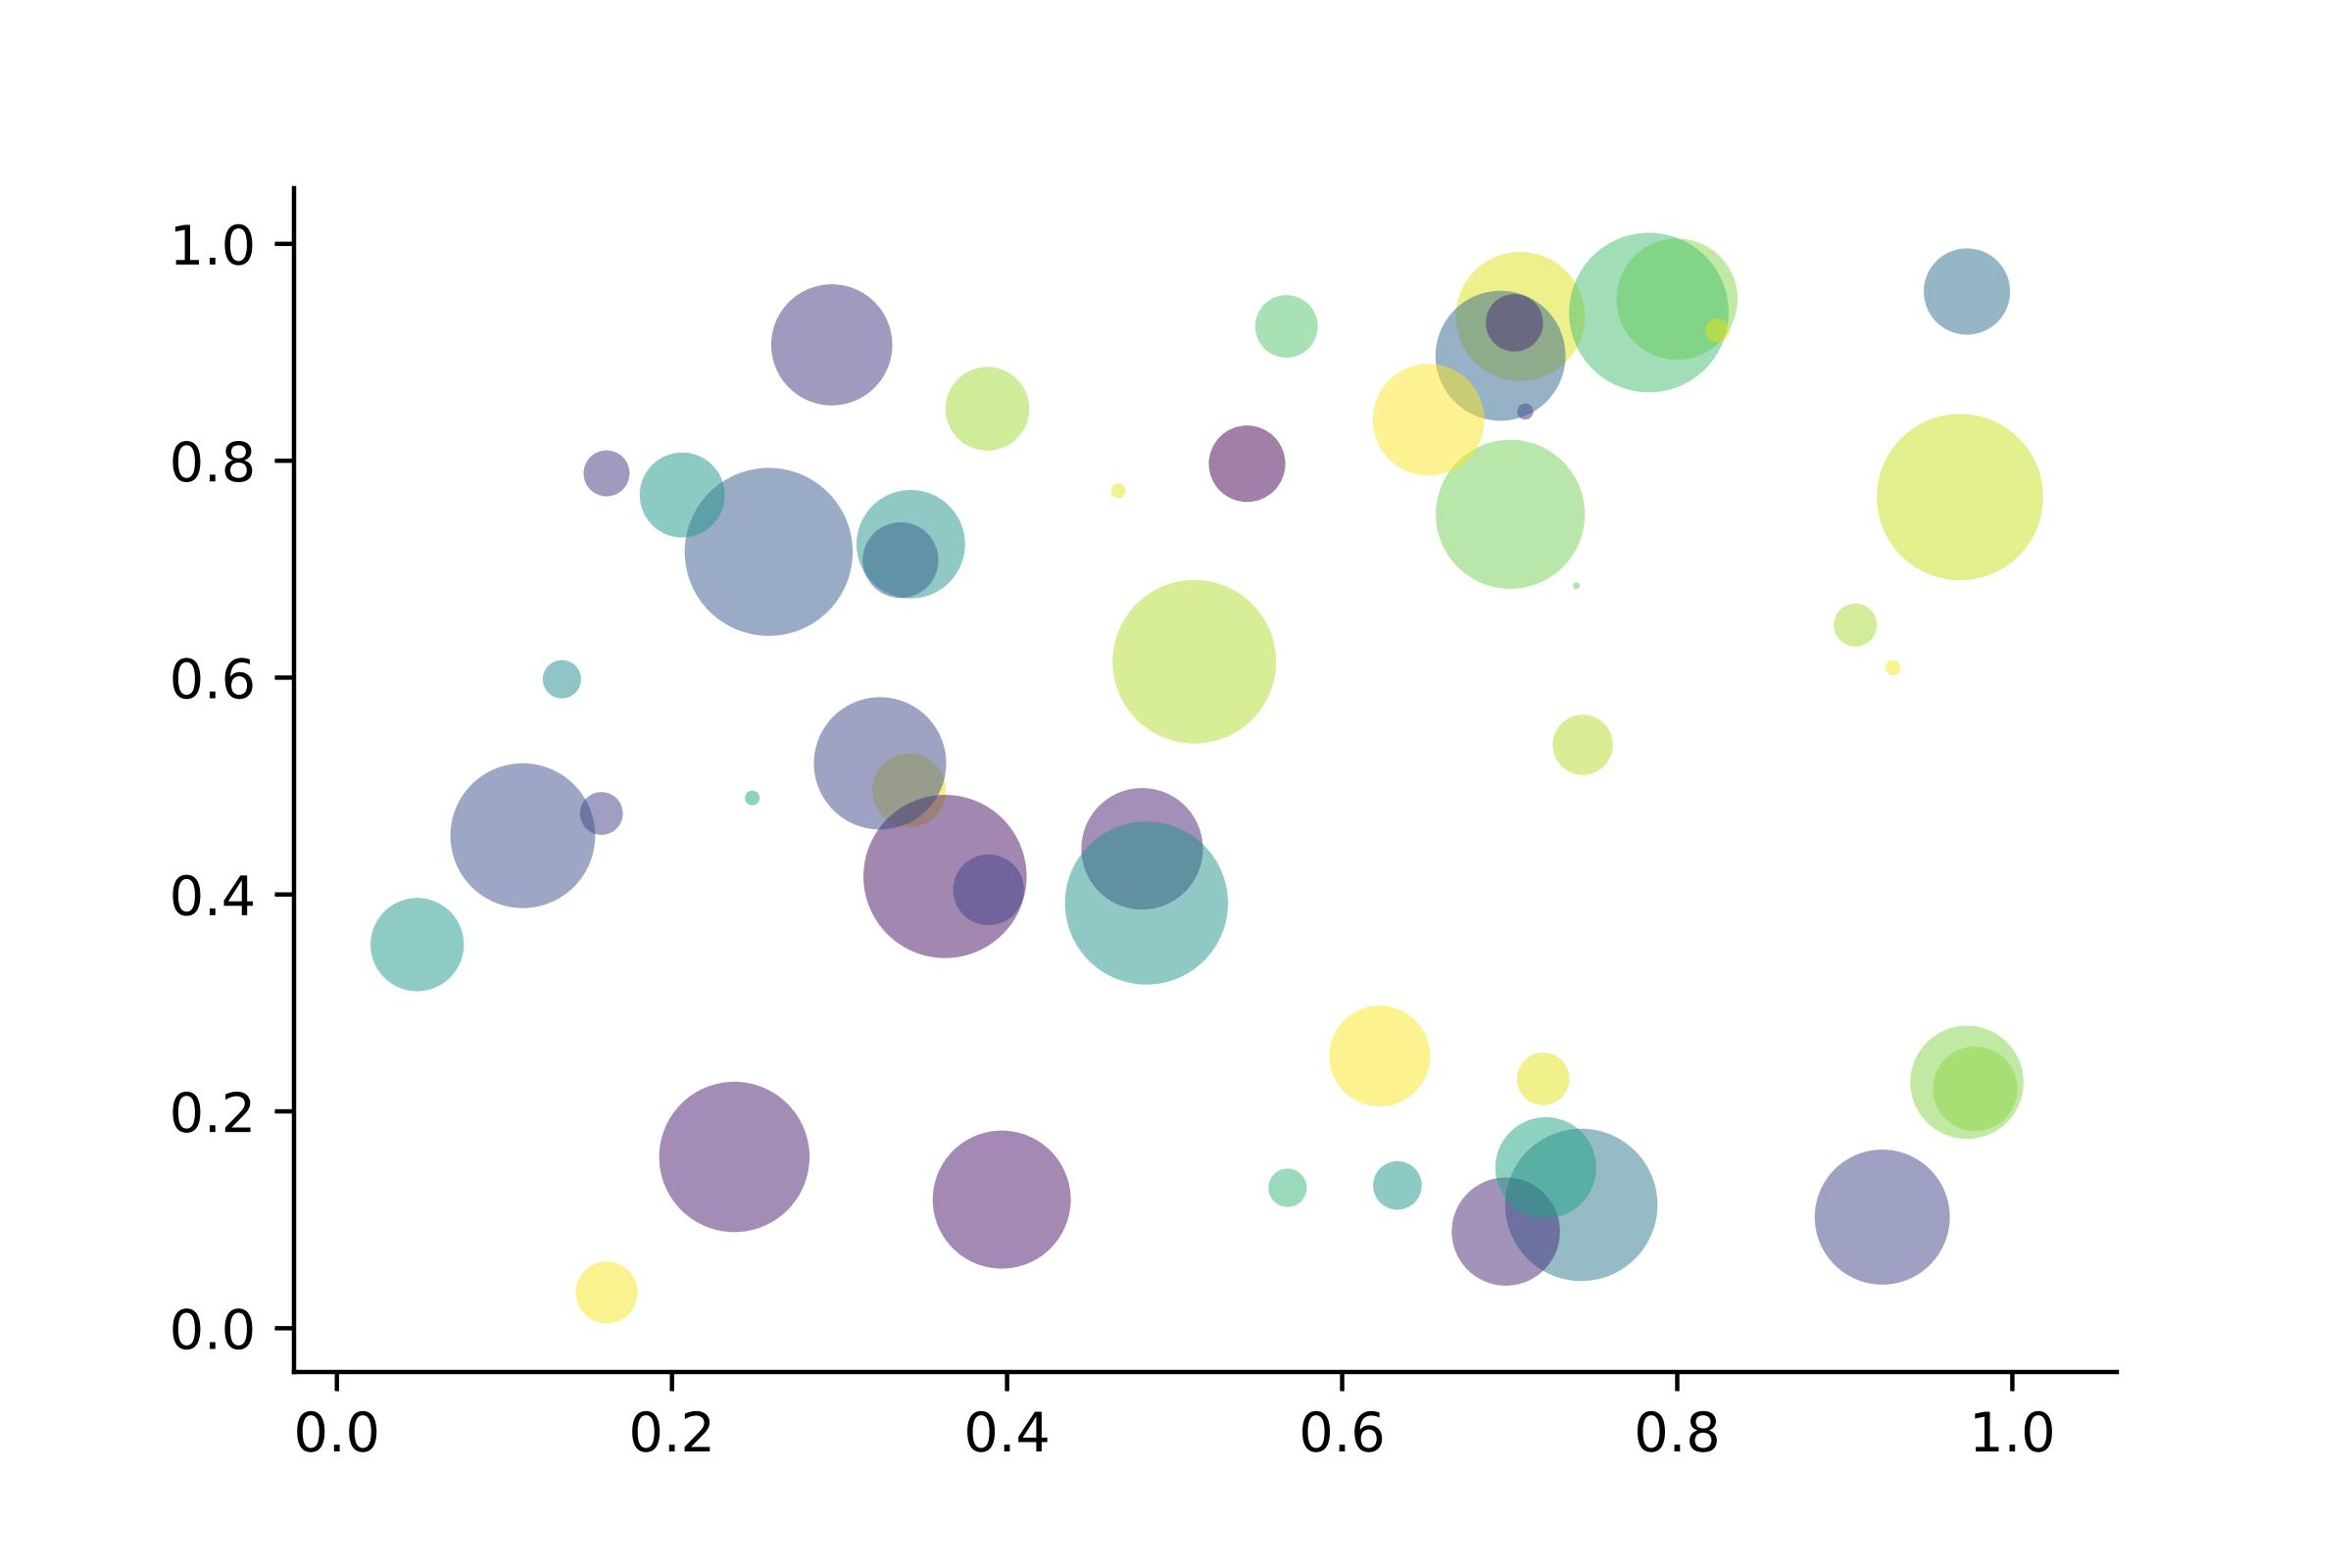
\includegraphics[width=0.6\textwidth]{scatter.jpg}
	\caption{散点图示例 $\hat{y}=a+bx$ \label{fig:scatter}}
\end{figure}

\begin{property}\label{property:cauchy}
	性质
	\begin{enumerate}
		\item 条目1
		\item 条目2
	\end{enumerate}
\end{property}

\begin{conclusion}
	结论
\end{conclusion}

\begin{example}
	例题
\end{example}

\begin{problemset}
	\item 练习1
	\item 练习2
	\item 练习3
\end{problemset}
	
\end{document}